% Apresentação final do TG2 -- estilo A (minimalista acadêmico). Roteiro: plano_apresentacao.md
\documentclass[aspectratio=169,11pt]{beamer}
\usepackage[brazilian]{babel}
\usepackage[T1]{fontenc}
\usepackage{lmodern}
\usepackage{amsmath}
\usepackage{booktabs}
\usepackage{tabularx}
\usepackage{tikz}
\usetikzlibrary{positioning,arrows.meta}
\usefonttheme{serif}
\graphicspath{{../Imagens/}}

\definecolor{azulita}{HTML}{0056B3}
\definecolor{cinza}{HTML}{555555}
\definecolor{fundocaixa}{HTML}{F2F6FB}

\setbeamertemplate{navigation symbols}{}
\setbeamercolor{frametitle}{fg=azulita}
\setbeamerfont{frametitle}{size=\Large,series=\bfseries}
\setbeamertemplate{frametitle}{\vspace*{0.25cm}\insertframetitle\par\vspace{2pt}{\color{azulita}\rule{\linewidth}{0.6pt}}}
\setbeamercolor{normal text}{fg=black}
\setbeamercolor{itemize item}{fg=azulita}
\setbeamertemplate{itemize item}{\small$\bullet$}
\setbeamertemplate{itemize subitem}{\scriptsize$\circ$}
\setbeamerfont{itemize/enumerate body}{size=\small}
\setbeamerfont{itemize/enumerate subbody}{size=\footnotesize}
\setbeamertemplate{footline}{\hspace{0.5cm}{\color{cinza}\tiny\insertsectionhead}\hfill{\color{cinza}\scriptsize\insertframenumber}\hspace{0.5cm}\vspace{0.3cm}}
\setlength{\leftmargini}{1.2em}

\newcolumntype{L}[1]{>{\raggedright\arraybackslash}p{#1}}
\newcolumntype{Y}{>{\raggedright\arraybackslash}X}
\newcommand{\fonte}[1]{\par\vspace{2pt}{\scriptsize\color{cinza}#1}}
\newenvironment{bullets}{\begin{itemize}\setlength{\itemsep}{5pt}}{\end{itemize}}
\newcommand{\caixa}[1]{\colorbox{fundocaixa}{\parbox{0.92\linewidth}{\centering #1}}}

\begin{document}

% =============================================================================
% CAPA
% =============================================================================
\begin{frame}[plain]
\centering

\includegraphics[height=1.2cm]{ita-logo.png}\par\vspace{0.4cm}
{\color{azulita}\large\bfseries Análise da influência de parâmetros de processo de fabricação (cinemáticos, de geometria da ferramenta, entre outros) na integridade de juntas soldadas por FSW\par}
\vspace{0.4cm}{\color{azulita}\rule{0.35\linewidth}{0.6pt}}\par\vspace{0.4cm}
{\normalsize Rafael Lucas de Albuquerque Louvain\par}\vspace{2pt}
{\small\color{cinza}Orientador: Prof. Dr. Lindolfo Araújo Moreira Filho\par}\vspace{0.3cm}
{\footnotesize\color{cinza}Trabalho de Graduação \;$\cdot$\; Engenharia Mecânica-Aeronáutica \;$\cdot$\; ITA \;$\cdot$\; 2026\par}
\end{frame}

% =============================================================================
\section{Introdução}
% =============================================================================
\begin{frame}{O processo FSW e sua relevância}
\begin{columns}[T,onlytextwidth]
\begin{column}{0.5\textwidth}
\begin{bullets}
  \item \textbf{Princípio:} uma ferramenta rotativa, formada por ombro e pino, gera calor por atrito e deformação plástica, amolece o metal e o mistura mecanicamente ao longo da junta.
  \item \textbf{Estado sólido:} como não há fusão, evitam-se as trincas de solidificação e a porosidade típicas da soldagem a arco.
  \item \textbf{Aplicações:} viabilizou ligas de alumínio 2xxx e 7xxx, antes consideradas de difícil soldagem; uso aeroespacial, naval e automotivo.
\end{bullets}
\end{column}
\begin{column}{0.47\textwidth}
\centering
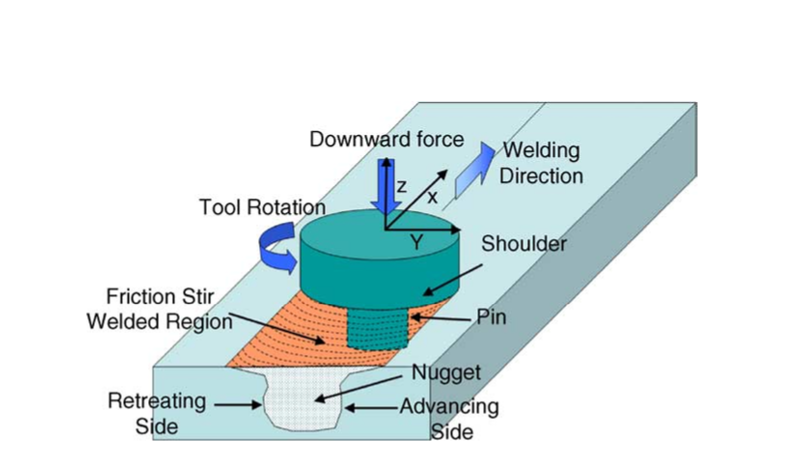
\includegraphics[width=\linewidth]{fig-esquema-processo-fsw.png}
\fonte{Mishra e Ma (2005)}
\end{column}
\end{columns}
\end{frame}

\begin{frame}{O problema: vazios volumétricos}
\begin{columns}[T,onlytextwidth]
\begin{column}{0.5\textwidth}
\begin{bullets}
  \item \textbf{O que é:} uma cavidade no interior da junta, em geral no lado de avanço, formada quando o material não preenche o espaço deixado pelo pino.
  \item \textbf{Por que preocupa:} atua como concentrador de tensão e reduz a resistência à tração e à fadiga da junta.
  \item \textbf{Difícil de detectar:} não aparece na superfície; exige ensaios não destrutivos (ultrassom, raio X) ou o corte da peça.
  \item \textbf{Consequência:} escolher parâmetros por tentativa e erro é caro; é preciso prever o defeito antes de soldar.
\end{bullets}
\end{column}
\begin{column}{0.47\textwidth}
\centering
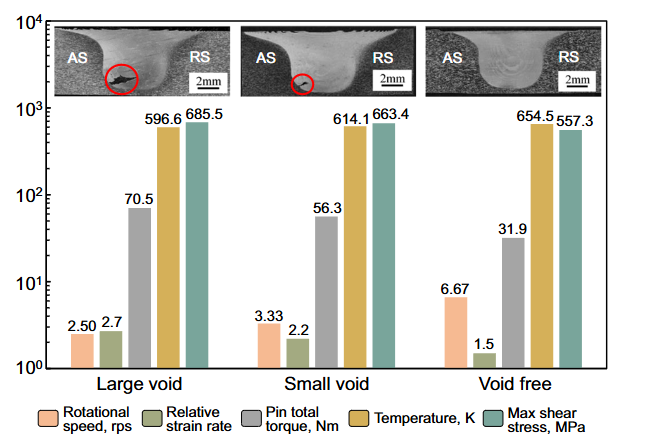
\includegraphics[width=\linewidth]{fig-vazio-variaveis-causais-du.png}
\fonte{Vazio grande, pequeno e sem vazio. Du, Mukherjee e DebRoy (2019)}
\end{column}
\end{columns}
\end{frame}

\begin{frame}{Como se prevê hoje}
\begin{bullets}
  \item \textbf{Simulação:} modelos de CFD e de elementos finitos descrevem o calor e o escoamento, mas exigem grande esforço computacional para cada condição.
  \item \textbf{Du, Mukherjee e DebRoy (2019):} compilaram 108 soldas da literatura e treinaram redes neurais e árvores de decisão para prever vazios.
  \item \textbf{Lacuna:} nenhum desses métodos fornece uma relação explícita, calculável à mão, entre os parâmetros e o defeito.
\end{bullets}
\vspace{0.1cm}
\centering\scriptsize\setlength{\tabcolsep}{4pt}
\begin{tabular}{cllc}
\toprule
\textbf{Método} & \textbf{Algoritmo} & \textbf{Entradas} & \textbf{Teste} \\ \midrule
1 & Rede neural & 10 parâmetros brutos de processo, geometria e material & 83,3\% \\
2 & Rede neural & Variáveis causais (modelo analítico) & 93,3\% \\
3 & Árvore de decisão & Variáveis causais (modelo analítico) & 90,0\% \\
4 & Rede neural & Variáveis causais (modelo numérico) & 96,6\% \\
5 & Árvore de decisão & Variáveis causais (modelo numérico) & 96,6\% \\ \bottomrule
\end{tabular}
\fonte{Du, Mukherjee e DebRoy (2019)}
\end{frame}

\begin{frame}{A linha de pesquisa no ITA}
\begin{bullets}
  \item \textbf{Cintra (2018):} soldou 47 condições de Alclad AA2024-T3, registrou defeitos de soldas quentes, frias e mistas e destacou a força de forjamento como parâmetro primordial.
  \item \textbf{Gomes (2019) e Esaki (2022):} modelagem térmica e por elementos finitos da temperatura de soldagem a partir dos ensaios de Cintra.
  \item \textbf{Batista Filho e Tanaka (2020) e Alcoforado (2021):} caracterização mecânica e metalográfica de juntas soldadas por FSW.
  \item \textbf{Bezerra (2025):} regressão logística da energia efetiva por comprimento sobre os ensaios de Cintra; concluiu que essa energia, isolada, não basta para separar soldas sãs e defeituosas.
  \item \textbf{Este trabalho:} combina variáveis de naturezas distintas e passa de uma liga e uma ferramenta para uma base com várias ligas, ferramentas e espessuras.
\end{bullets}
\end{frame}

\begin{frame}{Objetivos}
\vspace{0.3cm}
\begin{bullets}
  \item \textbf{Objetivo 1:} propor o Coeficiente Analítico de Vazio ($C_{void}$), uma expressão simples e explícita que preveja a ocorrência de vazios a partir dos parâmetros de processo, da geometria da ferramenta e das propriedades do material.
  \item \textbf{Meta:} atingir mais de 70\% de acurácia na previsão de vazios na base de 108 soldas de Du, Mukherjee e DebRoy (2019).
  \item \textbf{Objetivo 2:} hierarquizar a influência das naturezas das variáveis sobre a formação de vazios: cinemática, geométrica, térmica, dinâmica e metalúrgica.
\end{bullets}
\vspace{0.4cm}
\caixa{\small Substituir simulações e modelos de caixa-preta por uma equação aplicável no chão de fábrica.}
\end{frame}

% =============================================================================
\section{Revisão da literatura}
% =============================================================================
\begin{frame}{Ferramenta e variáveis do processo}
\begin{columns}[T,onlytextwidth]
\begin{column}{0.55\textwidth}
\begin{bullets}
  \item \textbf{Ferramenta:} o ombro (raio $R_s$) gera a maior parte do calor; o pino (raios $R_{pr}$ na raiz e $R_{pt}$ na ponta) arrasta e mistura o material.
  \item \textbf{Lados:} no lado de avanço, a velocidade da ferramenta soma-se à do avanço; no de recuo, subtrai-se; a solda é assimétrica.
  \item \textbf{Variáveis e naturezas:}
  \begin{itemize}
    \item cinemáticas: rotação $\omega$ e avanço $v$;
    \item geométricas: $R_s$, $R_{pr}$, $R_{pt}$ e espessura $t$;
    \item dinâmicas: pressão $p$ e inclinação $\theta$;
    \item térmica: difusividade $\alpha$; metalúrgica: limite de escoamento $\sigma_y$.
  \end{itemize}
\end{bullets}
\end{column}
\begin{column}{0.4\textwidth}
\centering
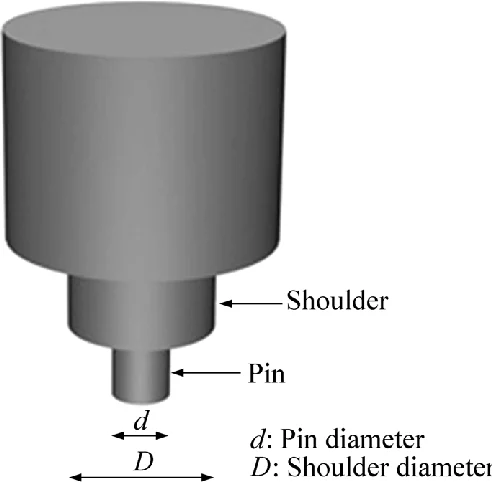
\includegraphics[width=0.8\linewidth]{fig-ferramenta-ombro-pino.png}
\fonte{Ferramenta: ombro (\textit{shoulder}) e pino (\textit{pin})}
\end{column}
\end{columns}
\end{frame}

\begin{frame}{Geração de calor e temperatura}
\begin{columns}[T,onlytextwidth]
\begin{column}{0.52\textwidth}
\begin{bullets}
  \item \textbf{Origem do calor:} atrito e deformação plástica na interface; o calor local é proporcional à velocidade de deslizamento $\omega r$, máxima na borda do ombro.
  \item \textbf{O ombro domina:} ferramentas com e sem pino produzem praticamente a mesma temperatura de pico.
  \item \textbf{Rotação × avanço:} a temperatura máxima é função forte da rotação; o avanço governa sobretudo a taxa de aquecimento.
  \item \textbf{Faixa típica:} pico entre 0,6 e 0,9 da temperatura de fusão; Arbegast e Hartley: $T/T_m = K(\omega^{2}/v)^{\alpha}$, com $\alpha \approx 0{,}05$.
\end{bullets}
\end{column}
\begin{column}{0.45\textwidth}
\centering
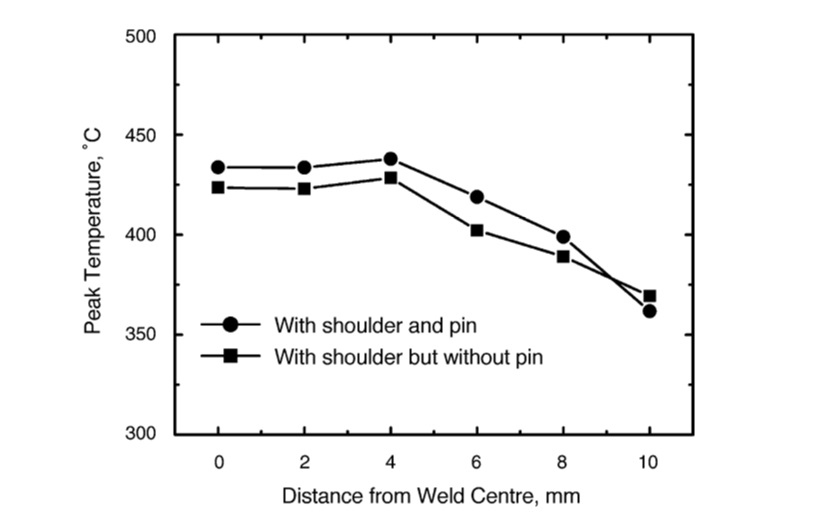
\includegraphics[width=\linewidth]{fig-temperatura-com-sem-pino.png}
\fonte{Temperatura de pico com e sem pino. Mishra e Ma (2005)}
\end{column}
\end{columns}
\end{frame}

\begin{frame}{Escoamento do material}
\begin{columns}[T,onlytextwidth]
\begin{column}{0.4\textwidth}
\begin{bullets}
  \item \textbf{Extrusão:} o material à frente da ferramenta é extrudado ao redor do pino, sobretudo pelo lado de recuo, e forjado atrás dela pela pressão do ombro.
  \item \textbf{Balanço de massa (Arbegast, 2008):} se o material que sai da frente do pino não for igual ao que retorna atrás dele, sobra uma cavidade: o vazio.
  \item \textbf{Geometria do pino:} pinos cônicos e com canais deslocam menos material e facilitam o transporte para baixo.
\end{bullets}
\end{column}
\begin{column}{0.57\textwidth}
\centering
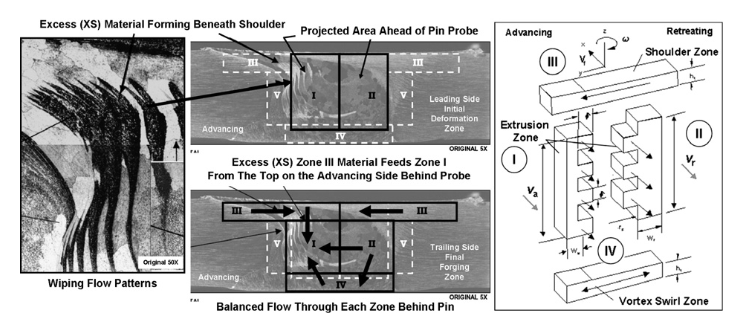
\includegraphics[width=\linewidth]{fig-zonas-escoamento-arbegast.png}
\fonte{Zonas de deformação do modelo de partição do escoamento. Arbegast (2008)}
\end{column}
\end{columns}
\end{frame}

\begin{frame}{Defeitos e a janela de processo}
\begin{columns}[T,onlytextwidth]
\begin{column}{0.44\textwidth}
\begin{bullets}
  \item \textbf{Lado frio} (rotação baixa, avanço alto): pouco calor e escoamento insuficiente; vazio e falta de preenchimento.
  \item \textbf{Lado quente} (rotação alta, avanço baixo): excesso de calor; rebarba, arrancamento superficial e colapso do núcleo.
  \item \textbf{Janela de processo:} entre os dois lados, soldas sãs; a força axial amplia essa janela.
  \item \textbf{O vazio é um defeito do lado frio.}
\end{bullets}
\end{column}
\begin{column}{0.53\textwidth}
\centering
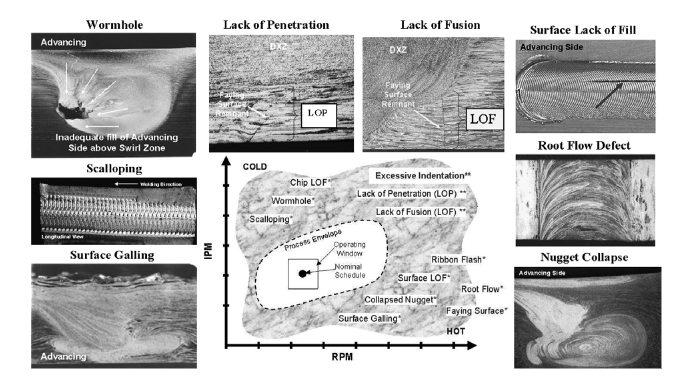
\includegraphics[width=\linewidth]{fig-tipos-defeitos-arbegast.png}
\fonte{Eixos: RPM, rotação; IPM, avanço. Arbegast (2008)}
\end{column}
\end{columns}
\end{frame}

\begin{frame}{Influência dos parâmetros}
\begin{columns}[T,onlytextwidth]
\begin{column}{0.52\textwidth}
\begin{bullets}
  \item \textbf{Rotação:} aumenta o calor e reduz o torque, com efeito que tende a saturar em rotações altas.
  \item \textbf{Avanço:} reduz o calor por comprimento de solda e aumenta as forças sobre a ferramenta.
  \item \textbf{Combinações clássicas:} avanço por rotação ($\omega/v$), pseudoíndice de calor ($\omega^{2}/v$) e energia por comprimento; cada uma atribui um peso diferente à rotação.
  \item \textbf{Raio do ombro:} principal fator geométrico do calor gerado; calor e torque crescem com $R_{s}^{3}$.
\end{bullets}
\end{column}
\begin{column}{0.45\textwidth}
\centering
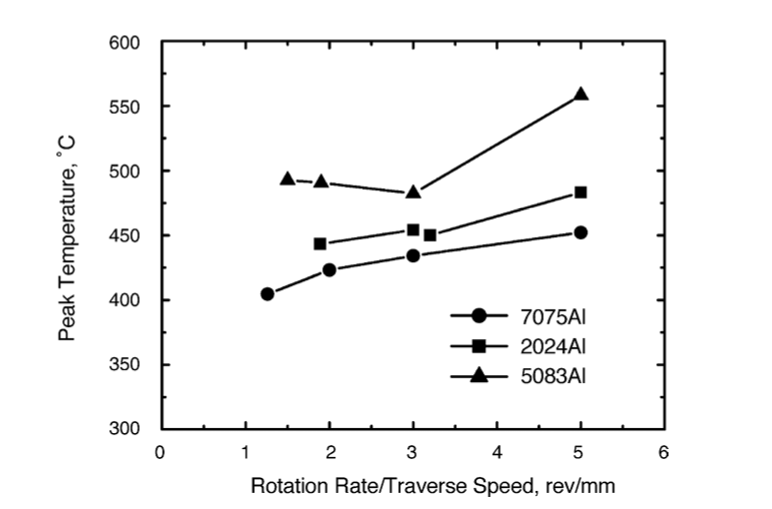
\includegraphics[width=\linewidth]{fig-temperatura-razao-rotacao-avanco.png}
\fonte{Temperatura de pico × razão rotação/avanço. Mishra e Ma (2005)}
\end{column}
\end{columns}
\end{frame}

\begin{frame}{Predição de vazios: Du, Mukherjee e DebRoy (2019)}
\begin{columns}[T,onlytextwidth]
\begin{column}{0.52\textwidth}
\begin{bullets}
  \item \textbf{Variáveis causais:} temperatura, taxa de deformação, torque e tensão de cisalhamento no pino, calculadas por modelos analíticos e numéricos.
  \item \textbf{Limites de decisão:} temperatura normalizada abaixo de 0,93 indicou tendência a vazio.
  \item \textbf{Hierarquia:} temperatura e tensão de cisalhamento $>$ torque $>$ taxa de deformação.
  \item \textbf{Aqui:} obter algo semelhante direto dos parâmetros, sem simulação.
\end{bullets}
\end{column}
\begin{column}{0.45\textwidth}
\centering
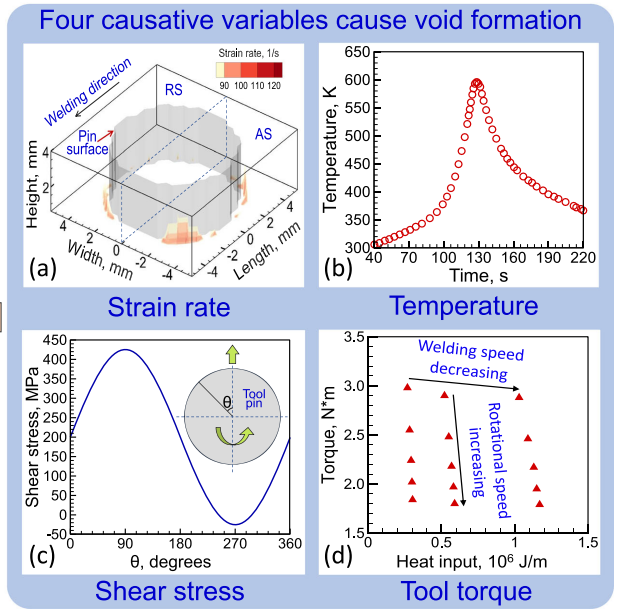
\includegraphics[height=5.3cm]{fig-variaveis-causais-du.png}
\fonte{Du, Mukherjee e DebRoy (2019)}
\end{column}
\end{columns}
\end{frame}

\begin{frame}{Síntese: o que esperar de cada variável}
\begin{bullets}
  \item \textbf{A revisão gera uma previsão do sinal de cada variável}, usada depois para conferir a coerência física dos modelos calibrados.
\end{bullets}
\vspace{0.05cm}
\centering\scriptsize
\begin{tabularx}{\textwidth}{L{3.6cm} Y L{3.6cm}}
\toprule
\textbf{Variável} & \textbf{Mecanismo principal} & \textbf{Efeito do aumento sobre o risco} \\ \midrule
Rotação, $\omega$ & Mais calor e mais material escoando & Reduz \\
Avanço, $v$ & Menos calor por comprimento; mais esforços & Aumenta (menos que $\omega$) \\
Raio do ombro, $R_s$ & Calor e torque $\propto R_{s}^{3}$; confinamento & Reduz \\
Raios do pino, $R_{pr}$, $R_{pt}$ & Volume varrido; conicidade & Incerto \\
Espessura, $t$ & Raiz mais distante do ombro e mais fria & Aumenta \\
Pressão axial, $p$ & Calor por atrito; forjamento & Reduz \\
Inclinação, $\theta$ & Forjamento na traseira da ferramenta & Reduz \\
Difusividade, $\alpha$ & Dissipação do calor gerado & Aumenta \\
Limite de escoamento, $\sigma_y$ & Resistência ao escoamento e calor por adesão & Incerto \\ \bottomrule
\end{tabularx}
\end{frame}

% =============================================================================
\section{Metodologia}
% =============================================================================
\begin{frame}{Visão geral}
\begin{bullets}
  \item \textbf{Um fluxo único}, aplicado de forma idêntica a todas as abordagens; cada abordagem nasceu do resultado da anterior.
  \item \textbf{Ao final}, o índice recomendado foi aplicado também aos ensaios de Cintra (2018), fora da base de calibração.
\end{bullets}
\vspace{0.2cm}
\centering
\begin{tikzpicture}[node distance=0.35cm,
  etapa/.style={draw, rounded corners=2pt, fill=gray!8, align=center, text width=2.9cm, minimum height=1.05cm, font=\scriptsize},
  modelo/.style={draw, rounded corners=2pt, fill=blue!6, align=center, text width=2.9cm, minimum height=1.05cm, font=\scriptsize},
  seta/.style={-{Stealth[length=1.8mm]}, thick}]
\node[etapa] (b) {\textbf{Base de dados}\\108 soldas, 14 estudos};
\node[etapa, right=of b] (t) {\textbf{Tratamento}\\SI; liga por $(\alpha,\sigma_y)$; valores assumidos};
\node[etapa, right=of t] (pi) {\textbf{Análise dimensional}\\7 grupos (teorema $\Pi$)};
\node[modelo, right=of pi] (ab) {\textbf{Abordagens}\\1: grupos $\Pi$\quad 2: $\omega R_s$\\3: $\omega R_s$ + grupos};
\node[etapa, below=0.6cm of ab] (c) {\textbf{Calibração}\\regressão logística; limiar no treino};
\node[etapa, left=of c] (v) {\textbf{Validação}\\protocolo de Du; 500 sorteios; por estudo};
\node[etapa, left=of v] (h) {\textbf{Diagnóstico}\\hierarquia das naturezas; robustez};
\node[etapa, left=of h] (ci) {\textbf{Aplicação}\\ensaios de Cintra (2018)};
\draw[seta] (b) -- (t); \draw[seta] (t) -- (pi); \draw[seta] (pi) -- (ab); \draw[seta] (ab) -- (c);
\draw[seta] (c) -- (v); \draw[seta] (v) -- (h); \draw[seta] (h) -- (ci);
\end{tikzpicture}
\end{frame}

\begin{frame}{Base de dados}
\begin{columns}[T,onlytextwidth]
\begin{column}{0.39\textwidth}
\begin{bullets}
  \item \textbf{Origem:} 108 soldas de topo de 14 estudos independentes, em AA2024, AA2219 e AA6061.
  \item \textbf{Saída:} 43 soldas com vazio e 65 sem.
  \item \textbf{Chave:} dentro de cada estudo só a rotação e o avanço variam; as outras oito variáveis são constantes.
  \item \textbf{Propriedades:} $\alpha$ e $\sigma_y$ têm um único valor por liga.
\end{bullets}
\end{column}
\begin{column}{0.59\textwidth}
\centering\scriptsize\setlength{\tabcolsep}{3pt}
\begin{tabular}{lll}
\toprule
\textbf{Variável} & \textbf{Faixa} & \textbf{Natureza} \\ \midrule
Avanço, $v$ & 15 a 1068 mm/min & Cinemática \\
Rotação, $\omega$ & 150 a 2500 rpm & Cinemática \\
Raio do ombro, $R_s$ & 5 a 14 mm & Geométrica \\
Raio do pino (raiz), $R_{pr}$ & 1,5 a 5,5 mm & Geométrica \\
Raio do pino (ponta), $R_{pt}$ & 0,9 a 4,2 mm & Geométrica \\
Espessura, $t$ & 2,1 a 17,5 mm & Geométrica \\
Difusividade, $\alpha$ & 4,9 a 6,9 mm$^2$/s & Térmica \\
Pressão axial, $p$ & 7,9 a 26,5 MPa & Dinâmica \\
Inclinação, $\theta$ & 2 a 2,5° & Dinâmica \\
Lim. de escoamento, $\sigma_y$ & 276 a 352 MPa & Metalúrgica \\ \bottomrule
\end{tabular}
\end{column}
\end{columns}
\end{frame}

\begin{frame}{Tratamento dos dados}
\vspace{0.2cm}
\begin{bullets}
  \item \textbf{Coluna de liga:} diverge das propriedades informadas em 33 das 108 linhas; como a difusividade e o limite de escoamento são coerentes com o estudo de origem, a liga passou a ser identificada pelo par $(\alpha, \sigma_y)$.
  \item \textbf{Valores assumidos:} quando o estudo de origem não informava, Du et al. adotaram valores usuais para a pressão (72 soldas) e a inclinação (71 soldas); esses valores foram marcados, e $\theta$ tem apenas dois valores, 2° e 2,5°.
  \item \textbf{Soldas duvidosas:} as linhas 84 a 89 estão atribuídas a um estudo de AA2024, mas trazem as propriedades da AA6061; foram mantidas e testadas na análise de robustez.
  \item \textbf{Unidades:} todas as grandezas foram convertidas para o Sistema Internacional.
\end{bullets}
\end{frame}

\begin{frame}{Análise dimensional e grupos adimensionais}
\begin{columns}[T,onlytextwidth]
\begin{column}{0.44\textwidth}
\begin{bullets}
  \item \textbf{Teorema $\Pi$:} 10 variáveis e 3 dimensões (massa, comprimento e tempo) resultam em 7 grupos adimensionais independentes.
  \item \textbf{Restrição 1:} a rotação só entra dividida por uma velocidade de referência: o avanço ($\omega R_s/v$) ou a difusão do calor ($\omega R_{s}^{2}/\alpha$).
  \item \textbf{Restrição 2:} $p$ e $\sigma_y$ só entram juntos, como $p/\sigma_y$; as naturezas dinâmica e metalúrgica não se separam.
\end{bullets}
\end{column}
\begin{column}{0.53\textwidth}
\centering\scriptsize\setlength{\tabcolsep}{4pt}
\begin{tabular}{cll}
\toprule
\textbf{Grupo} & \textbf{Expressão} & \textbf{Significado} \\ \midrule
$\Pi_1$ & $\omega R_s/v$ & Rotações por comprimento \\
$\Pi_2$ & $vR_s/\alpha$ & Número de Péclet \\
$\Pi_3$ & $p/\sigma_y$ & Pressão relativa \\
$\Pi_4$ & $t/R_s$ & Espessura relativa \\
$\Pi_5$ & $R_{pr}/R_s$ & Pino relativo ao ombro \\
$\Pi_6$ & $R_{pt}/R_{pr}$ & Conicidade do pino \\
$\Pi_7$ & $\theta$ & Inclinação \\ \bottomrule
\end{tabular}
\end{column}
\end{columns}
\end{frame}

\begin{frame}{Abordagem 1: produto de grupos adimensionais}
\begin{bullets}
  \item \textbf{Proposta original do TG1:} o índice é uma lei de potência dos grupos, com expoentes calibrados:
  \[ C_{void} = C_0 \prod_{i} \Pi_{i}^{\,\beta_i}, \qquad \text{vazio previsto se } C_{void} > 1. \]
  \item \textbf{Interpretação:} cada expoente indica o peso e o sentido da influência do seu grupo.
  \item \textbf{Três conjuntos de grupos}, cada um fundamentado em um mecanismo de formação de vazios:
\end{bullets}
\centering\scriptsize
\begin{tabularx}{\textwidth}{L{3.2cm} L{6.6cm} Y}
\toprule
\textbf{Conjunto} & \textbf{Grupos} & \textbf{Mecanismo} \\ \midrule
Buckingham completo & $\omega R_s/v$, $vR_s/\alpha$, $p/\sigma_y$, $t/R_s$, $R_{pr}/R_s$, $R_{pt}/R_{pr}$, $\theta$ & Todos os efeitos, um grupo cada \\
Conjunto térmico & $\omega R_{s}^{2}/\alpha$, $vR_s/\alpha$, $p/\sigma_y$, $t/R_s$ & Aporte de calor insuficiente \\
Conjunto escoamento & $\omega R_s/v$, $R_{pr}/R_s$, $R_{pt}/R_{pr}$, $t/R_{pr}$, $p/\sigma_y$ & Material insuficiente ao redor do pino \\ \bottomrule
\end{tabularx}
\end{frame}

\begin{frame}{Abordagem 2: índice físico único}
\begin{bullets}
  \item \textbf{Forma:} a razão entre uma velocidade crítica e a velocidade periférica do ombro:
  \[ C_{void} = \frac{V_{crit}}{\omega R_s}, \qquad \text{vazio previsto se } \omega R_s < V_{crit}. \]
  \item \textbf{Por que $\omega R_s$:} é a velocidade de deslizamento na borda do ombro, onde a geração de calor por unidade de área é máxima, e, em primeira aproximação, a velocidade do material arrastado pelo ombro.
  \item \textbf{Um único parâmetro:} apenas $V_{crit}$ é calibrado; não há expoentes ajustados.
  \item \textbf{Comparações:} as versões adimensionais $\omega R_s/v$ e $\omega R_{s}^{2}/\alpha$ e o índice formado apenas pela rotação.
\end{bullets}
\end{frame}

\begin{frame}{Abordagem 3: núcleo físico com termos complementares}
\vspace{0.2cm}
\begin{bullets}
  \item \textbf{Pergunta:} algum grupo adimensional acrescenta informação à velocidade periférica do ombro?
  \item \textbf{Forma:} o núcleo $\omega R_s$ multiplicado pelos grupos selecionados $S$:
  \[ C_{void} = C_0\,(\omega R_s)^{\beta_0} \prod_{j \in S} \Pi_{j}^{\,\beta_j}. \]
  \item \textbf{Seleção progressiva:} a cada passo, testa-se o acréscimo de cada um dos 7 grupos; um grupo só entra se aumentar a acurácia da validação interna em pelo menos 1 ponto percentual.
  \item \textbf{Sem olhar o teste:} toda a seleção é feita apenas com as soldas de treinamento.
\end{bullets}
\end{frame}

\begin{frame}{Calibração}
\begin{bullets}
  \item \textbf{Regressão logística = lei de potência:} o logaritmo da chance de vazio é linear nos logaritmos dos grupos, ou seja, a chance é um produto de potências, exatamente a forma do $C_{void}$:
  \[ \ln\!\left(\frac{P}{1-P}\right) = b_0 + \sum_i \beta_i \ln \Pi_i \quad \Longleftrightarrow \quad \frac{P}{1-P} = e^{b_0}\prod_i \Pi_{i}^{\,\beta_i}. \]
  \item \textbf{Classes equilibradas:} com 43 soldas com vazio e 65 sem, as duas classes recebem o mesmo peso total no ajuste.
  \item \textbf{Limiar:} escolhido exclusivamente no treinamento, como o valor que maximiza a acurácia.
  \item \textbf{Métricas:} acurácia (acertos totais), sensibilidade (vazios detectados) e especificidade (soldas sãs aprovadas).
\end{bullets}
\end{frame}

\begin{frame}{Protocolo de validação}
\begin{bullets}
  \item \textbf{Regra geral:} nenhuma decisão de modelagem (expoentes, limiar, termos) usa os dados de teste; divisões estratificadas, com 78 soldas de treinamento e 30 de teste.
\end{bullets}
\vspace{0.15cm}
\begin{columns}[T,onlytextwidth]
\begin{column}{0.32\textwidth}
\caixa{\small\textbf{Protocolo de Du et al.}}\par\vspace{4pt}
\scriptsize Um único sorteio 78/30, com semente fixada antes de qualquer modelagem. É o esquema comparável ao da referência.
\end{column}
\begin{column}{0.32\textwidth}
\caixa{\small\textbf{500 sorteios}}\par\vspace{4pt}
\scriptsize O mesmo procedimento repetido 500 vezes, recalibrando o modelo a cada vez. A média das acurácias é a medida principal, estatisticamente mais robusta.
\end{column}
\begin{column}{0.32\textwidth}
\caixa{\small\textbf{Validação por estudo}}\par\vspace{4pt}
\scriptsize Cada um dos 14 estudos sai inteiro para teste, e o modelo é calibrado com os demais. Simula uma máquina, uma ferramenta e uma chapa inéditas.
\end{column}
\end{columns}
\end{frame}

\begin{frame}{Hierarquia de influência e robustez}
\begin{bullets}
  \item \textbf{Sem um modelo específico:} a hierarquia vem de evidências simples, cada uma ligada a uma natureza.
  \item \textbf{Cinemática:} AUC calculada só com pares de soldas do mesmo estudo (fração de pares ordenada corretamente) e o expoente $c$ do avanço em $\omega\,v^{c}$.
  \item \textbf{Geométrica:} ganho de acurácia ao passar do índice $\omega$ para $\omega R_s$.
  \item \textbf{Dinâmica, metalúrgica e térmica:} efeito de retirar $p$ e $\theta$, frequência de escolha na abordagem 3 e desempenho das versões com $\alpha$.
  \item \textbf{Robustez:} todo o protocolo repetido sem $p$ e $\theta$ e sem as soldas duvidosas.
\end{bullets}
\end{frame}

\begin{frame}{Aplicação aos ensaios de Cintra (2018)}
\vspace{0.2cm}
\begin{bullets}
  \item \textbf{Objetivo:} verificar o comportamento do índice fora da base de calibração.
  \item \textbf{Ensaios:} 47 soldas de Alclad AA2024-T3, chapa de 3,2 mm, uma única ferramenta (ombro de 15,87 mm, pino de 6,4 mm); variam só a rotação (520 a 980 rpm) e o avanço (18 a 50 mm/min); defeito registrado: túnel.
  \item \textbf{Só a abordagem 2 se aplica:} as abordagens 1 e 3 exigiriam pressão, inclinação e raio da ponta do pino, não registrados ensaio a ensaio.
  \item \textbf{Dois testes:} o índice calibrado na base de Du aplicado diretamente; e o limiar recalibrado nos próprios ensaios (500 sorteios 33/14).
  \item \textbf{Ferramentas:} Python (NumPy, pandas, SciPy, scikit-learn, Matplotlib); código no repositório público do trabalho.
\end{bullets}
\end{frame}

% =============================================================================
\section{Resultados e discussão}
% =============================================================================
\begin{frame}{Caracterização da base}
\begin{columns}[T,onlytextwidth]
\begin{column}{0.4\textwidth}
\begin{bullets}
  \item \textbf{Diversidade:} espessuras de 2,1 a 17,5 mm, raios do ombro de 5 a 14 mm e rotações de 150 a 2500 rpm.
  \item \textbf{Dentro de cada estudo:} os vazios aparecem nas rotações mais baixas.
  \item \textbf{Entre estudos:} o nível de rotação em que o vazio desaparece muda, porque a ferramenta e a chapa mudam.
\end{bullets}
\end{column}
\begin{column}{0.57\textwidth}
\centering
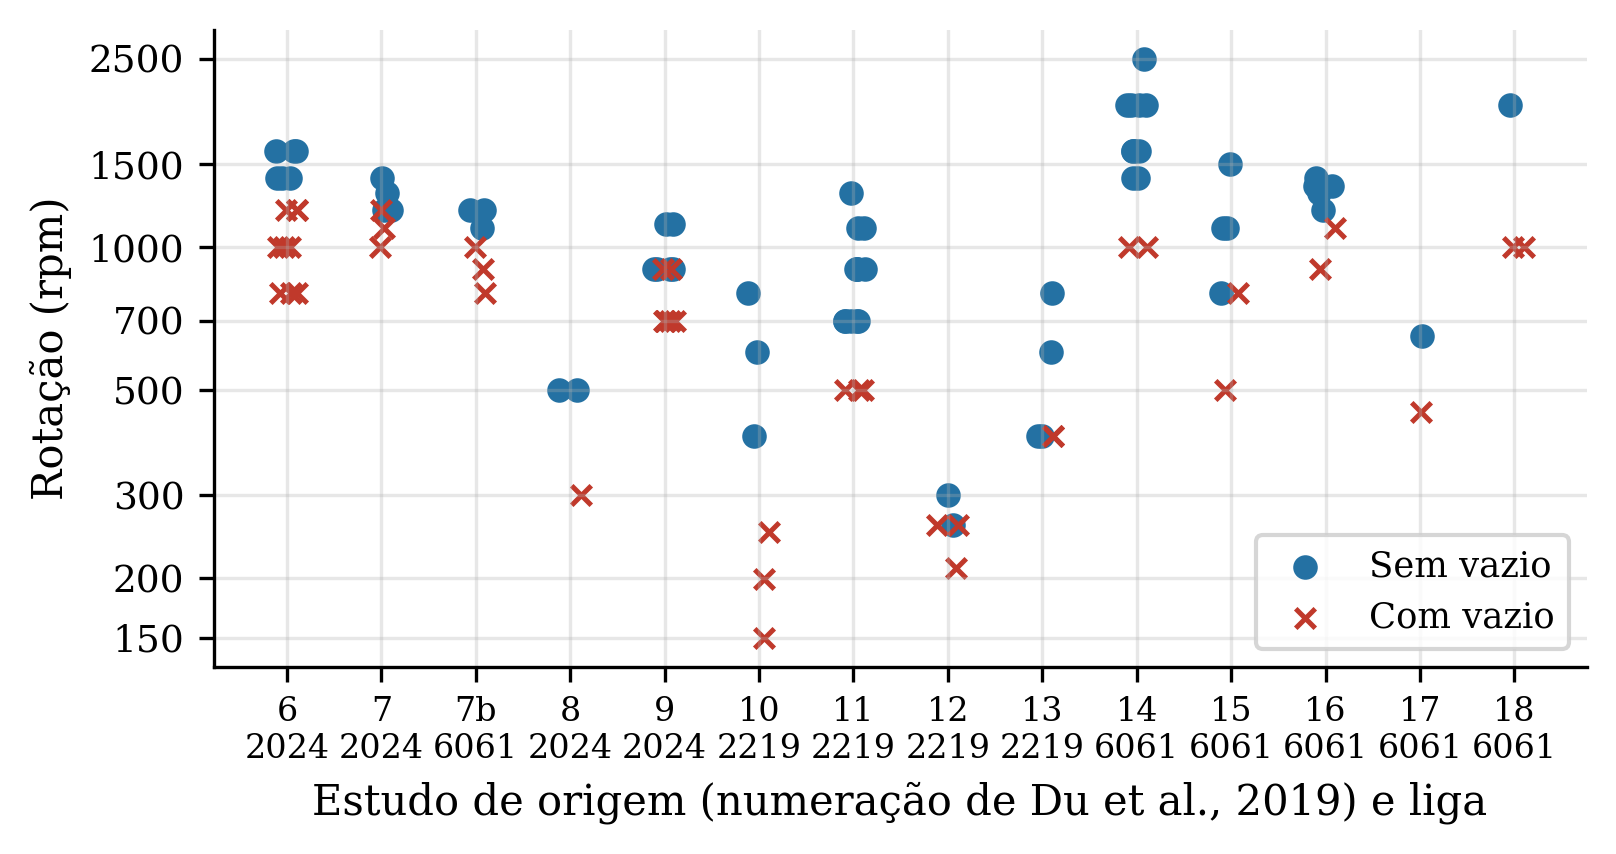
\includegraphics[width=\linewidth]{fig-r-rotacao-por-estudo.png}
\fonte{Rotação das soldas com e sem vazio em cada estudo}
\end{column}
\end{columns}
\end{frame}

\begin{frame}{Abordagem 1: desempenho}
\begin{bullets}
  \item \textbf{Protocolo de Du:} os três conjuntos atingem a meta (70,0\% a 83,3\%), e o Buckingham completo iguala a rede neural daqueles autores (83,3\%) com uma expressão explícita.
  \item \textbf{500 sorteios:} 60,7\% a 64,0\%, abaixo da meta no protocolo mais rigoroso.
  \item \textbf{Pista:} os conjuntos ficaram abaixo do índice formado só pela rotação (66,7\%): a informação estava concentrada na rotação.
\end{bullets}
\vspace{0.05cm}
\centering\scriptsize\setlength{\tabcolsep}{4pt}
\begin{tabular}{lcccccc}
\toprule
\textbf{Conjunto} & \textbf{Treino} & \textbf{Teste médio} & \textbf{Sens.} & \textbf{Espec.} & \textbf{Por estudo} & \textbf{Protocolo de Du} \\ \midrule
Buckingham completo & 74,4 & 63,2 & 54,6 & 68,8 & 54,6 & 83,3 \\
Conjunto térmico & 72,1 & 64,0 & 38,8 & 80,8 & 59,3 & 80,0 \\
Conjunto escoamento & 70,6 & 60,7 & 37,1 & 76,4 & 58,3 & 70,0 \\ \midrule
Classe majoritária & 60,3 & 60,0 & 0,0 & 100,0 & 60,2 & 60,0 \\
Apenas a rotação & 70,8 & 66,7 & 75,4 & 60,9 & 63,0 & 60,0 \\ \bottomrule
\end{tabular}
\end{frame}

\begin{frame}{Por que os grupos falharam: o regime de condução}
\begin{bullets}
  \item \textbf{Número de Péclet:} $vR_s/\alpha < 1$ em 93\% das soldas (mediana de 0,30).
  \item \textbf{Significado:} o calor se difunde à frente da ferramenta mais depressa do que ela avança; o campo de temperatura é quase estacionário em relação à ferramenta.
  \item \textbf{Consequência:} a temperatura junto ao ombro depende da potência gerada (função de $\omega$ e $R_s$), e não da energia por comprimento; por isso, dividir a rotação pelo avanço ou por $\alpha/R_s$ piora o índice.
\end{bullets}
\vspace{0.1cm}
\centering\footnotesize
\begin{tabular}{lccc}
\toprule
\textbf{Índice} & \textbf{Treino} & \textbf{Teste médio} & \textbf{Por estudo} \\ \midrule
Velocidade periférica do ombro, $\omega R_s$ & 76,8 & 72,9 & 66,7 \\
$\omega R_s$ dividida pelo avanço, $\omega R_s/v$ & 66,3 & 60,9 & 59,3 \\
$\omega R_s$ dividida pela escala de difusão, $\omega R_{s}^{2}/\alpha$ & 69,2 & 63,7 & 59,3 \\ \bottomrule
\end{tabular}
\end{frame}

\begin{frame}{Rotação × avanço dentro dos estudos}
\begin{columns}[T,onlytextwidth]
\begin{column}{0.45\textwidth}
\begin{bullets}
  \item \textbf{Comparação justa:} só pares de soldas do mesmo estudo, uma com e outra sem vazio.
  \item \textbf{AUC:} a rotação ordena corretamente 96\% dos pares; o avanço, sozinho, 54\%, praticamente um sorteio.
  \item \textbf{Expoente do avanço:} em $\omega\,v^{c}$, o melhor valor é $c = -0{,}10$ (IC de 95\%: $-0{,}30$ a $+0{,}05$), cerca de um décimo do peso da rotação.
  \item \textbf{Literatura descartada:} o intervalo exclui $\omega/v$ ($c=-1$) e $\omega^{2}/v$ ($c=-0{,}5$).
\end{bullets}
\end{column}
\begin{column}{0.52\textwidth}
\centering
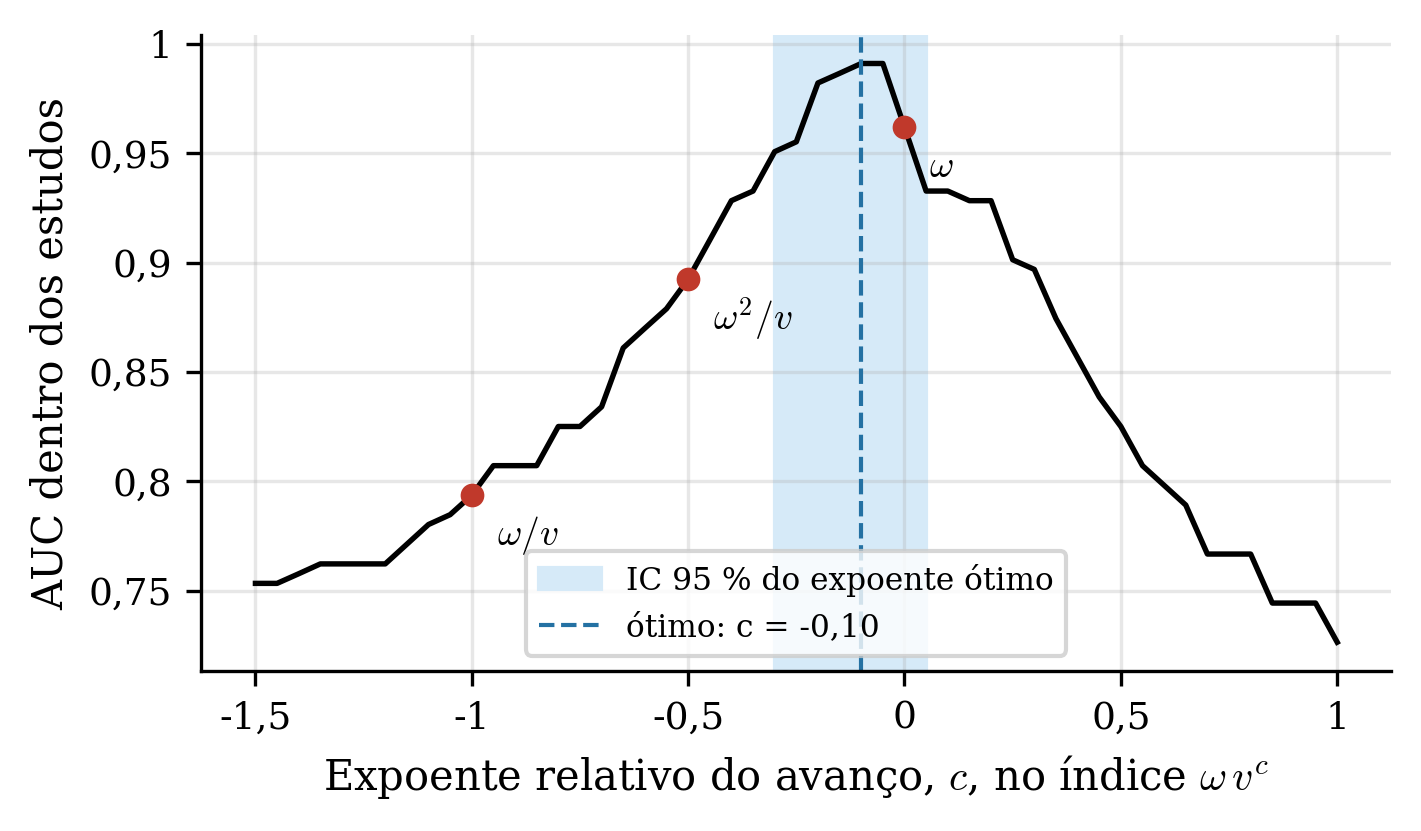
\includegraphics[width=\linewidth]{fig-r-auc-intra-avanco.png}
\fonte{AUC dentro dos estudos em função do expoente do avanço}
\end{column}
\end{columns}
\end{frame}

\begin{frame}{Abordagem 1: expressões calibradas}
\begin{bullets}
  \item \textbf{Calibração:} expoentes ajustados nas 78 soldas de treinamento do protocolo de Du et al.; prevê-se vazio quando $C_{void} > 1$.
  \item \textbf{Leitura:} expoente negativo indica que aumentar o grupo reduz o risco; todos os conjuntos atribuem à rotação, via $\omega R_s/v$ ou $\omega R_s^2/\alpha$, o sentido esperado.
\end{bullets}
\footnotesize
\begin{align*}
C_{void}^{(\text{Buckingham})} &= C_0 \left(\tfrac{\omega R_s}{v}\right)^{-1{,}25}\left(\tfrac{vR_s}{\alpha}\right)^{-0{,}82}\left(\tfrac{p}{\sigma_y}\right)^{-1{,}37}\left(\tfrac{t}{R_s}\right)^{-0{,}42}\left(\tfrac{R_{pr}}{R_s}\right)^{-1{,}82}\left(\tfrac{R_{pt}}{R_{pr}}\right)^{-0{,}42}\theta^{-0{,}39} \\[4pt]
C_{void}^{(\text{térmico})} &= C_0 \left(\tfrac{\omega R_{s}^{2}}{\alpha}\right)^{-1{,}07}\left(\tfrac{vR_s}{\alpha}\right)^{0{,}26}\left(\tfrac{p}{\sigma_y}\right)^{-1{,}32}\left(\tfrac{t}{R_s}\right)^{-0{,}74} \\[4pt]
C_{void}^{(\text{escoamento})} &= C_0 \left(\tfrac{\omega R_s}{v}\right)^{-0{,}70}\left(\tfrac{R_{pr}}{R_s}\right)^{-2{,}98}\left(\tfrac{R_{pt}}{R_{pr}}\right)^{-0{,}10}\left(\tfrac{t}{R_{pr}}\right)^{-0{,}46}\left(\tfrac{p}{\sigma_y}\right)^{-1{,}74}
\end{align*}
\end{frame}

\begin{frame}{Coerência física dos expoentes}
{\small Conjunto térmico calibrado (o de melhor desempenho na abordagem 1):}
\[ C_{void} = C_0 \left(\frac{\omega R_{s}^{2}}{\alpha}\right)^{-1{,}07}\left(\frac{vR_s}{\alpha}\right)^{0{,}26}\left(\frac{p}{\sigma_y}\right)^{-1{,}32}\left(\frac{t}{R_s}\right)^{-0{,}74} \]
\begin{columns}[T,onlytextwidth]
\begin{column}{0.52\textwidth}
\begin{bullets}
  \item \textbf{Coerentes:} rotação, raio do ombro, pressão e difusividade têm o sinal esperado; o avanço também, com peso pequeno (+0,26).
  \item \textbf{Exceção:} a espessura sai com sinal oposto ao esperado, pois só varia entre estudos, que diferem também em ferramenta e rotação.
\end{bullets}
\end{column}
\begin{column}{0.45\textwidth}
\centering\scriptsize\setlength{\tabcolsep}{3pt}
\begin{tabular}{lccc}
\toprule
\textbf{Variável} & \textbf{Expoente} & \textbf{Esperado} & \textbf{Confere} \\ \midrule
$\omega$ & $-1{,}07$ & $-$ & Sim \\
$v$ & $+0{,}26$ & $+$ & Sim \\
$R_s$ & $-1{,}13$ & $-$ & Sim \\
$t$ & $-0{,}74$ & $+$ & Não \\
$\alpha$ & $+0{,}81$ & $+$ & Sim \\
$p$ & $-1{,}32$ & $-$ & Sim \\
$\sigma_y$ & $+1{,}32$ & Incerto & n/a \\ \bottomrule
\end{tabular}
\end{column}
\end{columns}
\end{frame}

\begin{frame}{Abordagem 2: velocidade periférica crítica do ombro}
\begin{columns}[T,onlytextwidth]
\begin{column}{0.47\textwidth}
\begin{bullets}
  \item \textbf{Índice:} $C_{void} = V_{crit}/(\omega R_s)$; prevê-se vazio quando $\omega R_s < V_{crit}$, isto é, quando falta calor junto ao ombro.
  \item \textbf{Limiar calibrado:} $V_{crit} = 0{,}84$~m/s, ou rotação (rpm) $\times$ raio do ombro (mm) $\approx 8.000$.
  \item \textbf{Desempenho:} 90,0\% no protocolo de Du et al. (27 de 30 soldas) e 72,9\% na média de 500 sorteios, acima da meta nos dois.
  \item \textbf{Simplicidade:} um único parâmetro, sem simulação; o avanço e a pressão não entram na expressão.
\end{bullets}
\end{column}
\begin{column}{0.5\textwidth}
\centering
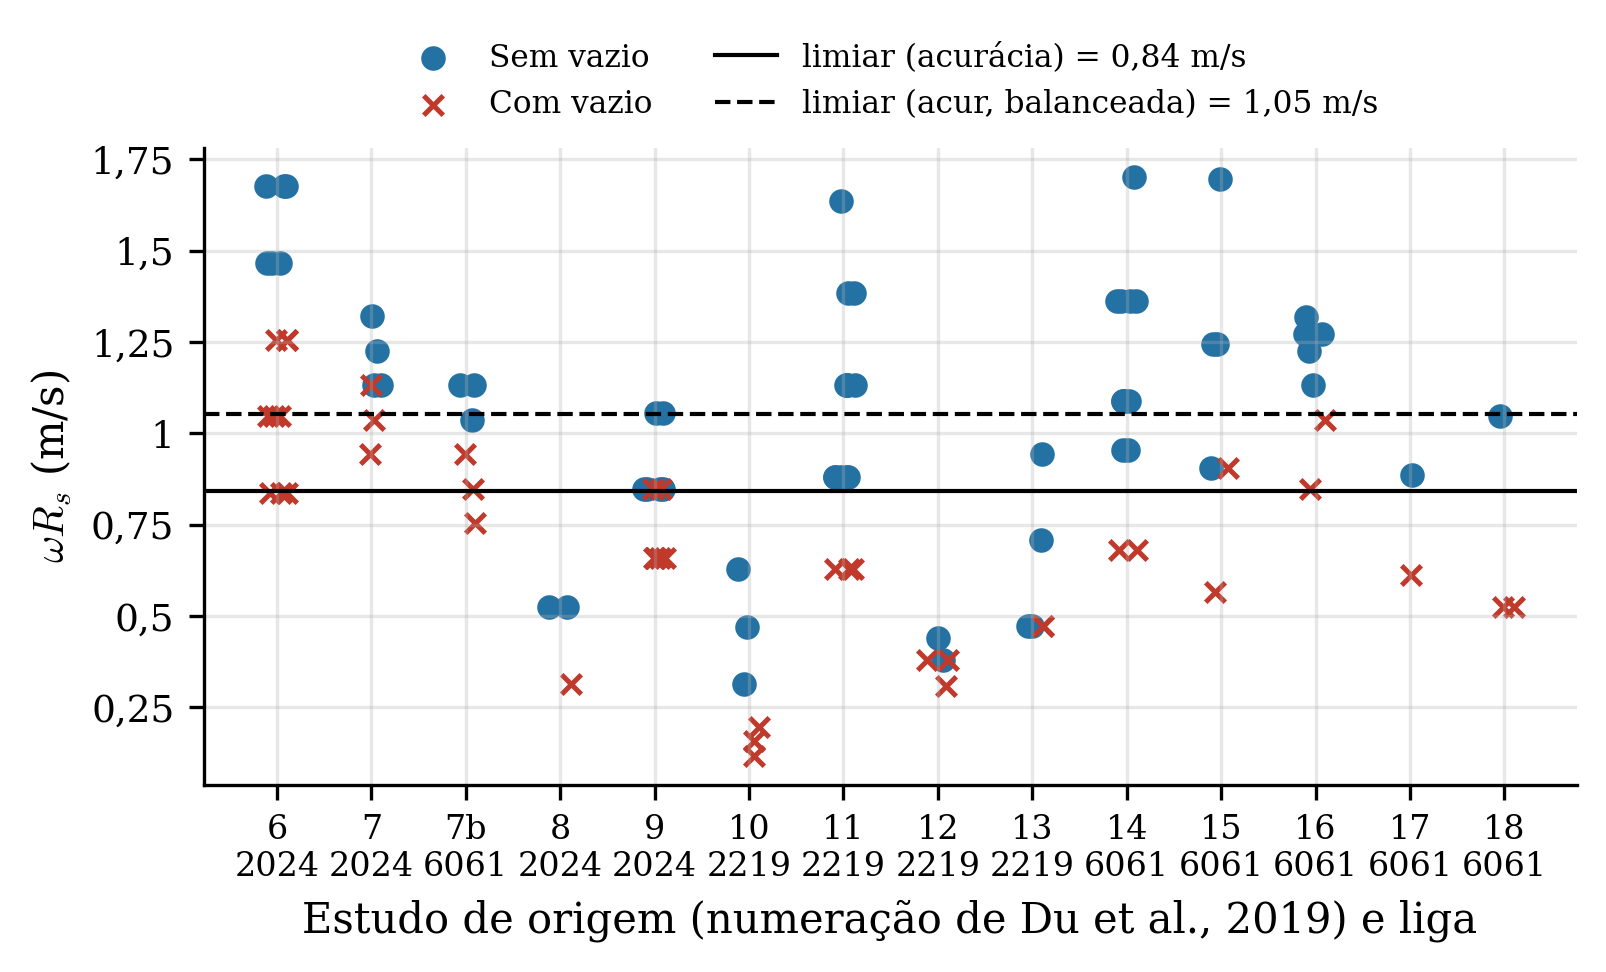
\includegraphics[width=\linewidth]{fig-r-indice-wrs.png}
\fonte{Soldas abaixo da linha cheia: vazio previsto.}
\end{column}
\end{columns}
\end{frame}

\begin{frame}{Como usar na prática}
\begin{bullets}
  \item \textbf{Exemplo, ombro de 10 mm:} a 600 rpm, $\omega R_s \approx 0{,}63$~m/s e $C_{void} \approx 1{,}3 > 1$, vazio previsto; a 1.200 rpm, $\omega R_s \approx 1{,}26$~m/s e $C_{void} \approx 0{,}67$, solda sã.
  \item \textbf{Rotação mínima:} para essa ferramenta, cerca de 800 rpm; um ombro maior atinge a mesma velocidade com menos rotação.
  \item \textbf{Uso industrial:} como aprovar uma solda com vazio é o erro mais grave, sugere-se o limiar conservador de 1,05~m/s ($\approx 10.000$ rpm$\cdot$mm), que detecta três de cada quatro vazios.
\end{bullets}
\vspace{0.1cm}
\centering\scriptsize\setlength{\tabcolsep}{4pt}
\begin{tabular}{lcccccc}
\toprule
\textbf{Limiar} & \textbf{$V_{crit}$ (m/s)} & \textbf{Teste médio} & \textbf{Sens.} & \textbf{Espec.} & \textbf{Por estudo} & \textbf{Protocolo de Du} \\ \midrule
Máxima acurácia & 0,84 & 72,9 & 63,0 & 79,4 & 66,7 & 90,0 \\
Conservador & 1,05 & 70,3 & 74,9 & 67,2 & 64,8 & 86,7 \\ \bottomrule
\end{tabular}
\end{frame}

\begin{frame}{Abordagem 3: núcleo físico com termos complementares}
\begin{columns}[T,onlytextwidth]
\begin{column}{0.52\textwidth}
\begin{bullets}
  \item \textbf{Ganho pequeno:} a acurácia média passou de 72,9\% para 74,0\%; na validação por estudo, nenhum ganho (66,7\%).
  \item \textbf{Sobreajuste:} a acurácia de treinamento subiu de 76,8\% para 81,2\%, aumentando a distância entre treino e teste.
  \item \textbf{Instabilidade:} em média só 1,3 termo entra, e o conjunto escolhido muda de sorteio para sorteio.
  \item \textbf{Conclusão:} não justifica a complexidade adicional; a abordagem 2 é a recomendada.
\end{bullets}
\end{column}
\begin{column}{0.45\textwidth}
\centering\scriptsize
\begin{tabular}{llc}
\toprule
\textbf{Grupo} & \textbf{Natureza} & \textbf{Freq.} \\ \midrule
$R_{pt}/R_{pr}$ & Geométrica & 57\% \\
$p/\sigma_y$ & Dinâmica e metalúrgica & 30\% \\
$\theta$ & Dinâmica & 19\% \\
$t/R_s$ & Geométrica & 15\% \\
$R_{pr}/R_s$ & Geométrica & 4\% \\
$vR_s/\alpha$ & Cin., geom. e térmica & 4\% \\
$\omega R_s/v$ & Cin. e geométrica & 1\% \\ \midrule
Nenhum & & 15\% \\ \bottomrule
\end{tabular}
\fonte{Frequência de escolha nos 500 sorteios}
\end{column}
\end{columns}
\end{frame}

\begin{frame}{Comparação com Du et al.: mesmo protocolo}
\begin{columns}[T,onlytextwidth]
\begin{column}{0.44\textwidth}
\begin{bullets}
  \item \textbf{Abordagem 2 (90,0\%):} acima da rede neural com os mesmos parâmetros (83,3\%).
  \item \textbf{Igual à árvore de decisão} baseada em variáveis causais de um modelo analítico (90,0\%).
  \item \textbf{A cerca de 6 pontos} dos métodos com variáveis de simulação numérica (96,6\%), sem nenhuma simulação.
  \item \textbf{Ressalva:} os conjuntos de teste não são os mesmos; a leitura é de desempenhos da mesma ordem.
\end{bullets}
\end{column}
\begin{column}{0.53\textwidth}
\centering
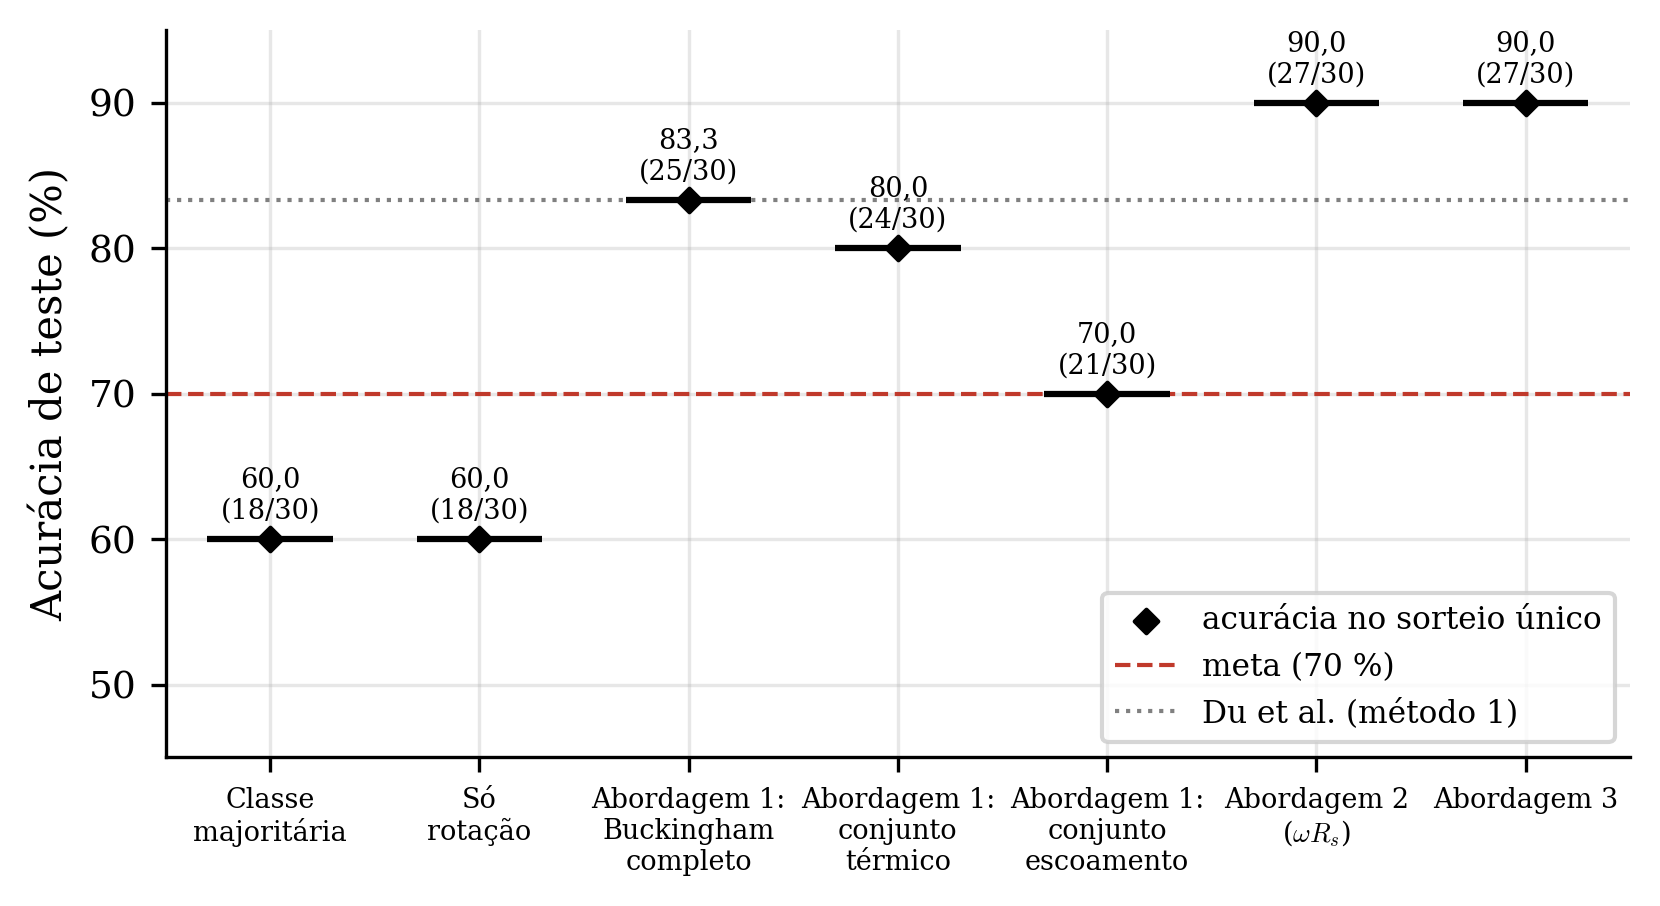
\includegraphics[width=\linewidth]{fig-r-comparacao-protocolo-du.png}
\fonte{Acurácia no sorteio único (protocolo de Du et al.)}
\end{column}
\end{columns}
\end{frame}

\begin{frame}{Comparação no protocolo rigoroso}
\begin{columns}[T,onlytextwidth]
\begin{column}{0.44\textwidth}
\begin{bullets}
  \item \textbf{Médias nos 500 sorteios:} abordagem 2 com 72,9\%, abordagem 3 com 74,0\% e abordagem 1 entre 60,7\% e 64,0\%.
  \item \textbf{Um sorteio engana:} para o mesmo modelo, um único sorteio varia de cerca de 60\% a 83\%; o sorteio do protocolo de Du ficou no percentil 99.
  \item \textbf{Generalização:} 66,7\% na validação por estudo, a 3,3 pontos da meta mesmo em máquinas, ferramentas e chapas inteiramente novas.
\end{bullets}
\end{column}
\begin{column}{0.53\textwidth}
\centering
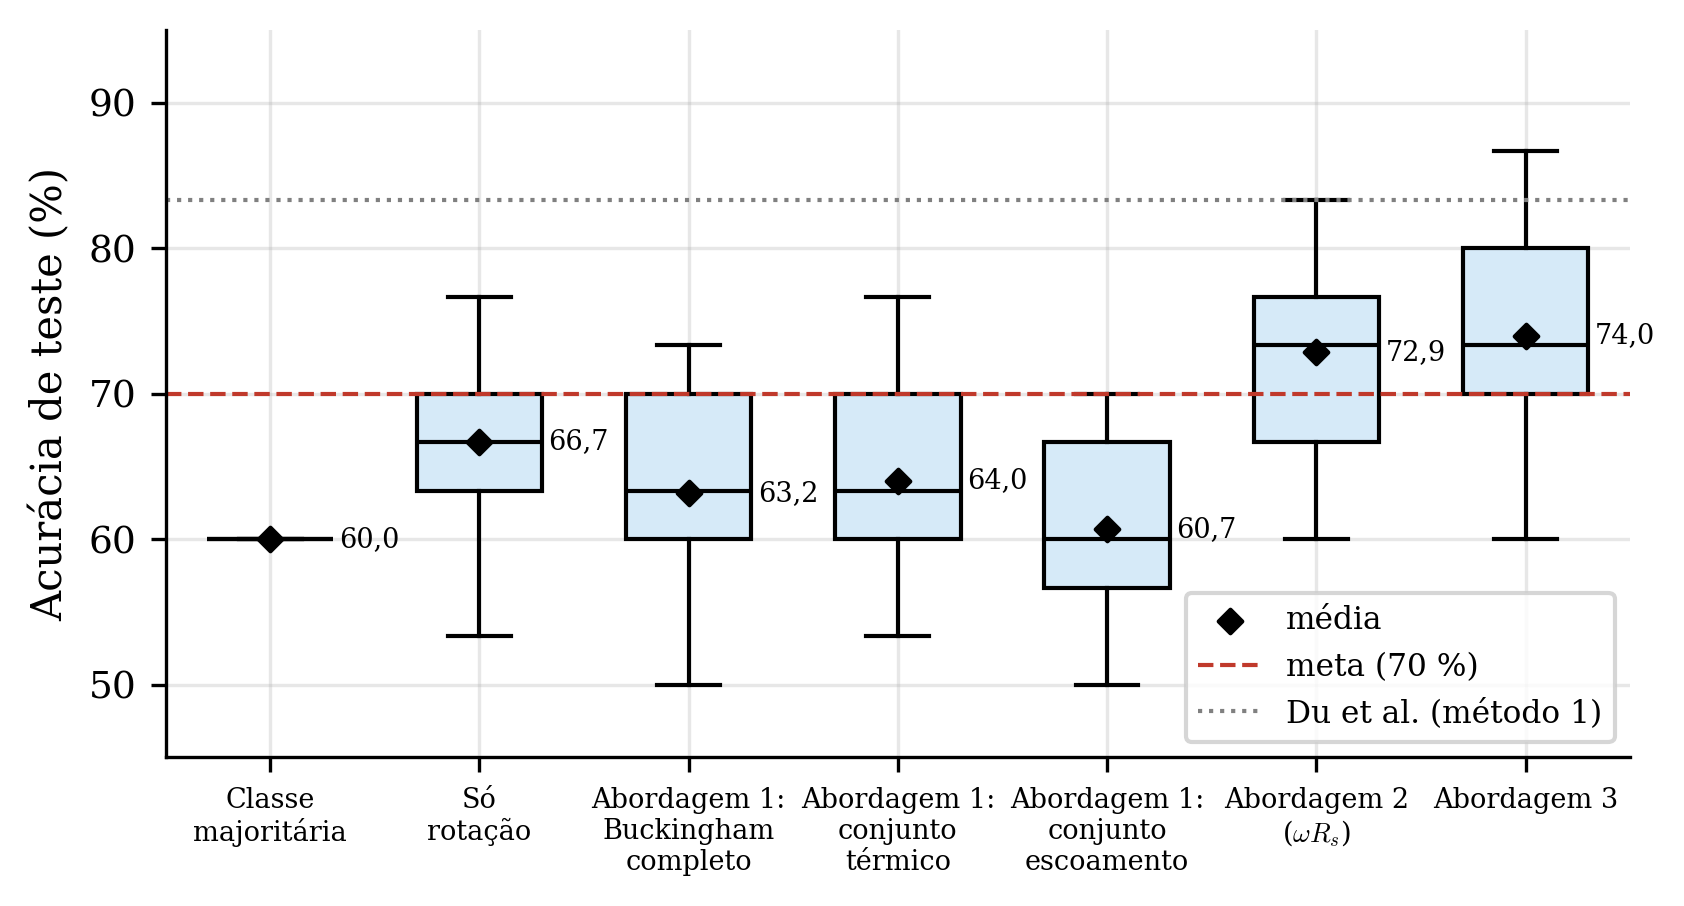
\includegraphics[width=\linewidth]{fig-r-comparacao-abordagens.png}
\fonte{Distribuição da acurácia de teste nos 500 sorteios}
\end{column}
\end{columns}
\end{frame}

\begin{frame}{Os dois protocolos lado a lado}
\begin{bullets}
  \item \textbf{Mesmos modelos, mesma base:} à esquerda, a distribuição nos 500 sorteios; à direita, o sorteio único do protocolo de Du et al.
  \item \textbf{O sorteio único favorece todos os modelos:} cada um aparece bem acima da sua média, o que mostra por que a média de muitos sorteios é a medida principal.
\end{bullets}
\vspace{0.1cm}
\begin{columns}[T,onlytextwidth]
\begin{column}{0.49\textwidth}
\centering
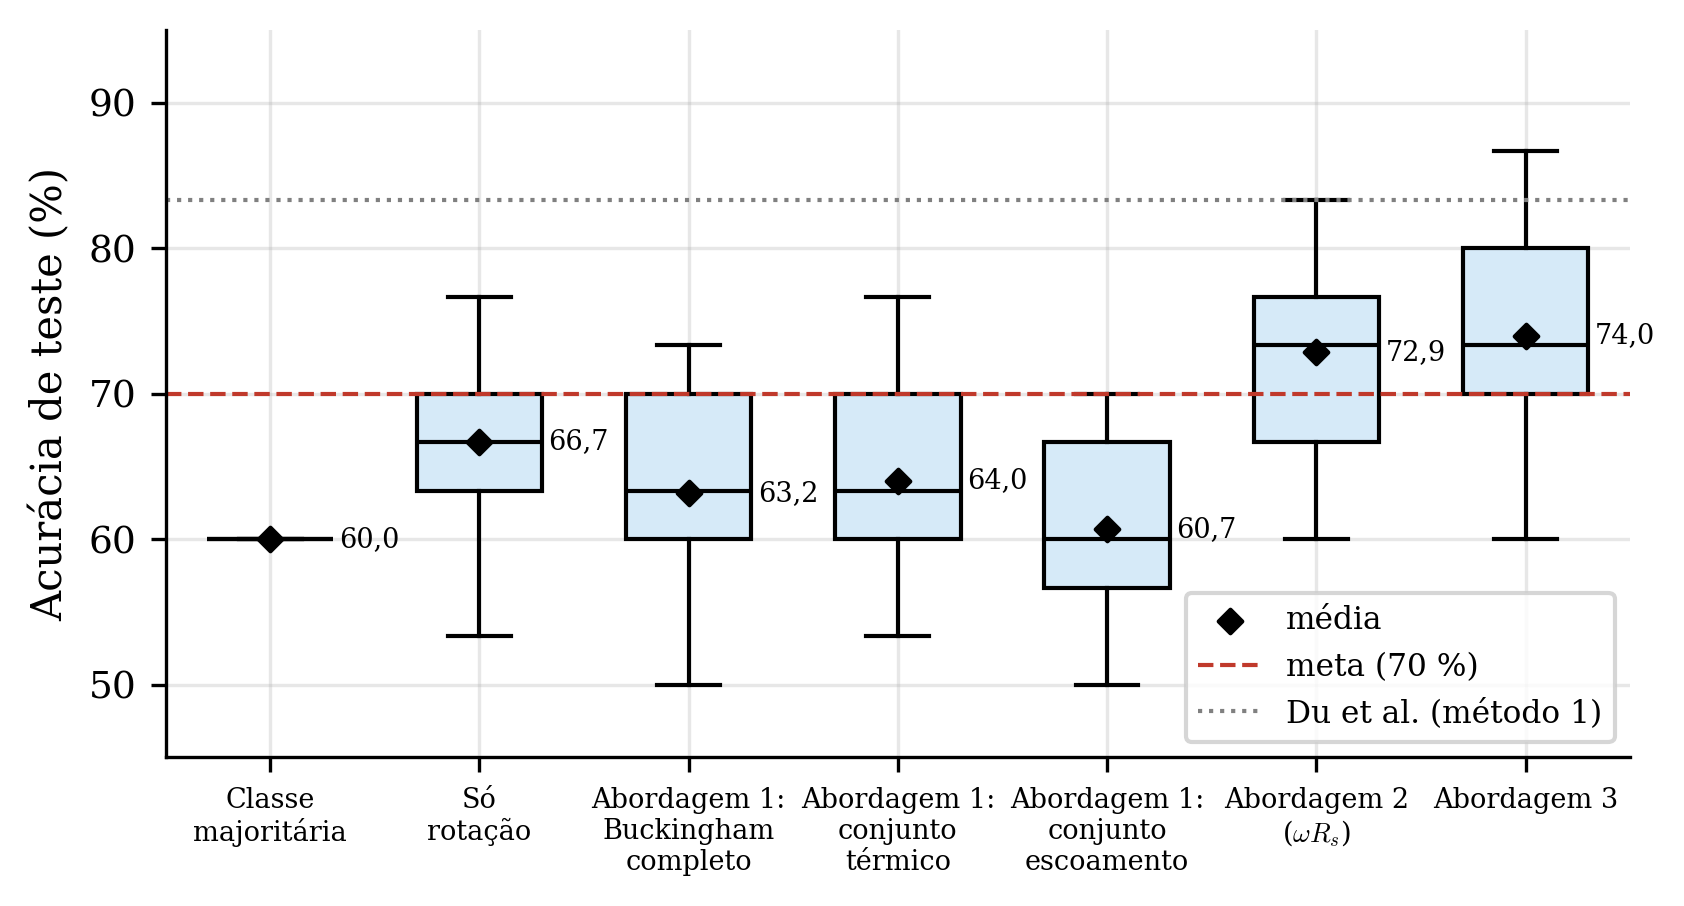
\includegraphics[width=0.93\linewidth]{fig-r-comparacao-abordagens.png}
\fonte{500 sorteios (protocolo principal)}
\end{column}
\begin{column}{0.49\textwidth}
\centering
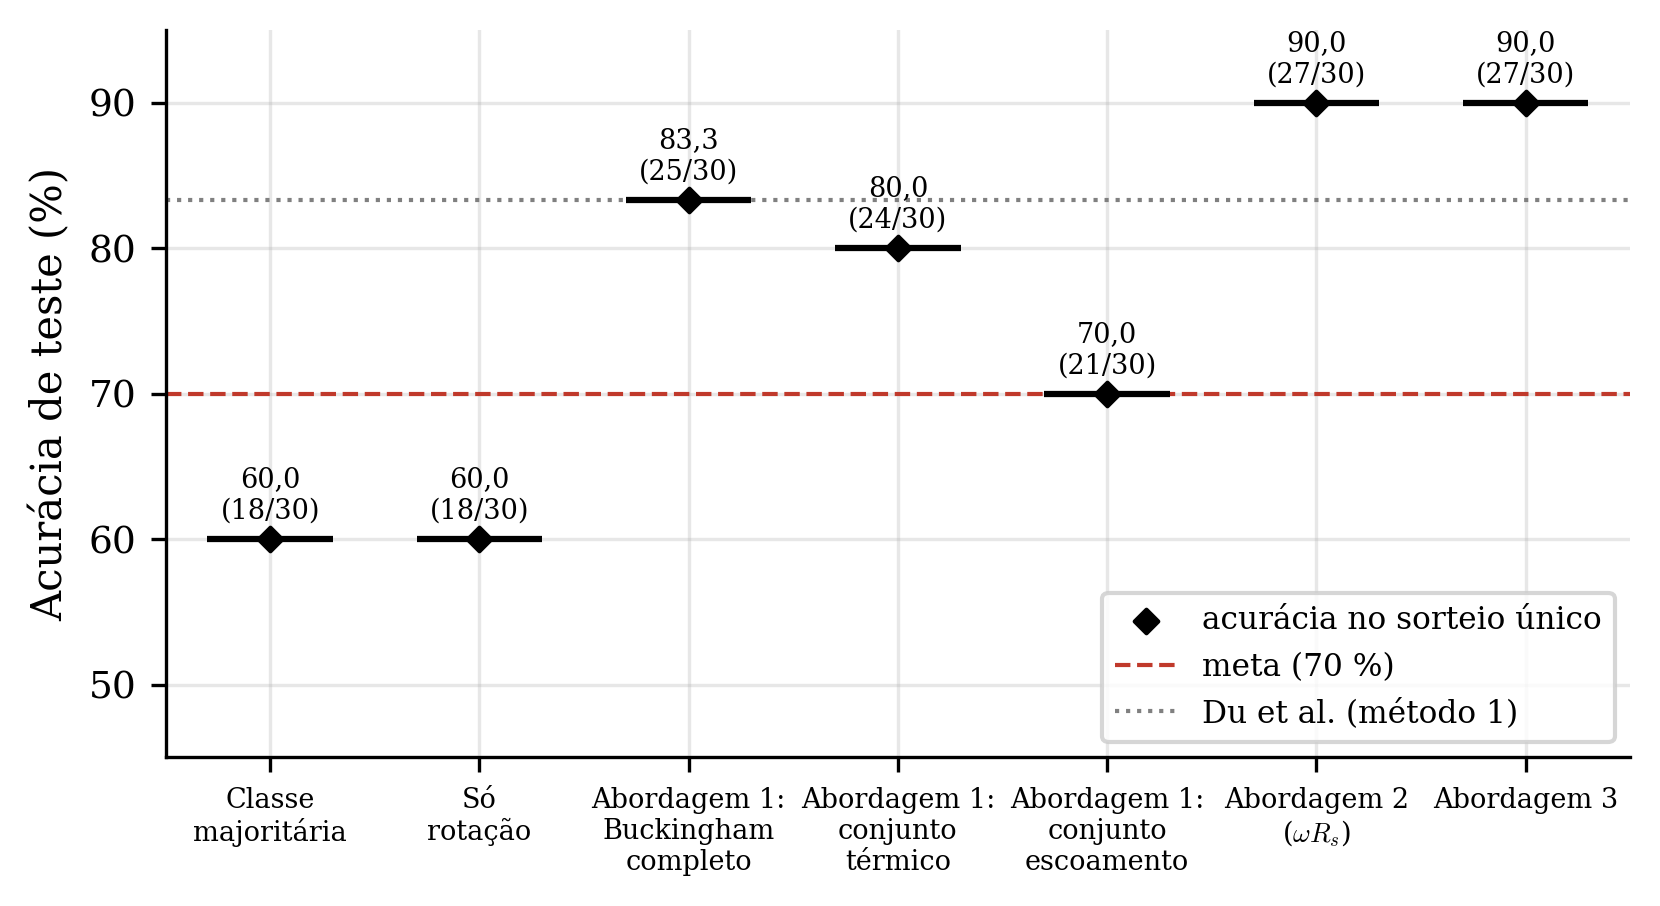
\includegraphics[width=0.93\linewidth]{fig-r-comparacao-protocolo-du.png}
\fonte{Sorteio único (protocolo de Du et al.)}
\end{column}
\end{columns}
\end{frame}

\begin{frame}{Hierarquia das naturezas}
\vspace{0.1cm}
\begin{bullets}
  \item \textbf{1. Cinemática (rotação):} dentro dos estudos, a rotação ordena 96\% dos pares; o avanço, 54\%.
  \item \textbf{2. Geométrica (raio do ombro):} acrescentar $R_s$ à rotação eleva a acurácia de 66,7\% para 72,9\%; a conicidade do pino é o termo mais escolhido na abordagem 3.
  \item \textbf{3. Dinâmica e metalúrgica ($p/\sigma_y$):} escolhida em 30\% dos sorteios da abordagem 3, mas retirá-la quase não altera o desempenho.
  \item \textbf{4. Térmica ($\alpha$):} incluir a difusividade piora o índice (de 72,9\% para 63,7\%).
  \item \textbf{Ressalva:} como $p$ e $\theta$ foram assumidos e $\alpha$ e $\sigma_y$ têm um valor por liga, efeitos não detectados não são necessariamente desprezíveis; a hierarquia vale para a fronteira fria.
\end{bullets}
\end{frame}

\begin{frame}{Robustez dos resultados}
\begin{bullets}
  \item \textbf{Sem $p$ e $\theta$:} a abordagem 2, que não usa essas variáveis, fica inalterada; a abordagem 3 perde 0,3 ponto e a abordagem 1, de 0,7 a 2,2 pontos.
  \item \textbf{Sem as linhas 84 a 89:} as abordagens 2 e 3 melhoram ligeiramente, em especial na validação por estudo.
  \item \textbf{Conclusão:} as conclusões não dependem dos dados mais incertos da base.
\end{bullets}
\vspace{0.1cm}
\centering\scriptsize\setlength{\tabcolsep}{4pt}
\begin{tabular}{lccc}
\toprule
\textbf{Modelo} & \textbf{Base completa} & \textbf{Sem $p$ e $\theta$} & \textbf{Sem as linhas 84--89} \\ \midrule
Abordagem 1: Buckingham completo & 63,2 (54,6) & 61,6 (50,9) & 62,6 (53,9) \\
Abordagem 1: conjunto térmico & 64,0 (59,3) & 61,8 (50,9) & 63,4 (54,9) \\
Abordagem 1: conjunto escoamento & 60,7 (58,3) & 60,0 (55,6) & 61,7 (59,8) \\
Abordagem 2 & 72,9 (66,7) & 72,9 (66,7) & 74,1 (71,6) \\
Abordagem 3 & 74,0 (66,7) & 73,7 (66,7) & 76,8 (72,5) \\ \bottomrule
\end{tabular}
\fonte{Acurácia de teste média; entre parênteses, validação por estudo}
\end{frame}

\begin{frame}{Vazios de origem fria na base de Du et al.}
\begin{columns}[T,onlytextwidth]
\begin{column}{0.52\textwidth}
\begin{bullets}
  \item \textbf{Fonte:} Du et al. atribuem os vazios a aporte de calor insuficiente, por baixa rotação, ombro inadequado ou chapa espessa.
  \item \textbf{Dados:} a fração de soldas com vazio cai à medida que $\omega R_s$ aumenta, e nenhuma solda acima de 1,3 m/s tem vazio.
  \item \textbf{Dentro dos estudos:} em 96\% dos pares, a solda com vazio é a de menor rotação.
  \item \textbf{Leitura:} no regime frio, a velocidade periférica concentra o poder de previsão, associada a um limiar de calor insuficiente.
\end{bullets}
\end{column}
\begin{column}{0.45\textwidth}
\centering\scriptsize\setlength{\tabcolsep}{4pt}
\begin{tabular}{cccc}
\toprule
\textbf{$\omega R_s$ (m/s)} & \textbf{Soldas} & \textbf{Vazio} & \textbf{Fração} \\ \midrule
até 0,50 & 15 & 9 & 60,0\% \\
0,50 a 0,84 & 22 & 18 & 81,8\% \\
0,84 a 1,05 & 28 & 12 & 42,9\% \\
1,05 a 1,30 & 26 & 4 & 15,4\% \\
acima de 1,30 & 17 & 0 & 0,0\% \\ \bottomrule
\end{tabular}
\fonte{Primeira faixa: soldas sãs de chapas grossas de AA2219}
\end{column}
\end{columns}
\end{frame}

\begin{frame}{Ensaios de Cintra (2018): um mecanismo diferente}
\begin{columns}[T,onlytextwidth]
\begin{column}{0.55\textwidth}
\begin{bullets}
  \item \textbf{Aplicação direta:} todas as soldas ficam abaixo do limiar ($\approx 1.010$ rpm com essa ferramenta), e 83\% têm túnel: coerente, mas igual a prever sempre vazio.
  \item \textbf{Mas a rotação não separa:} a fração com túnel não cai com a rotação, e nenhuma recalibração do limiar separa as soldas.
  \item \textbf{Leitura:} soldas quentes ou mistas, atribuídas por Cintra à variação da força de forjamento; defeito limitado pela consolidação.
  \item \textbf{Implicação:} nesse regime, a pressão axial e a inclinação tendem a ser mais relevantes que $\omega R_s$.
\end{bullets}
\end{column}
\begin{column}{0.42\textwidth}
\centering\scriptsize\setlength{\tabcolsep}{4pt}
\begin{tabular}{cccc}
\toprule
\textbf{rpm} & \textbf{$\omega R_s$ (m/s)} & \textbf{Ensaios} & \textbf{Túnel} \\ \midrule
520 & 0,43 & 7 & 71,4\% \\
635 & 0,53 & 19 & 78,9\% \\
810 & 0,67 & 15 & 93,3\% \\
980 & 0,81 & 6 & 83,3\% \\ \midrule
Total & --- & 47 & 83,0\% \\ \bottomrule
\end{tabular}
\fonte{Ensaios de Cintra (2018) por rotação}
\end{column}
\end{columns}
\end{frame}

\begin{frame}{Limitações}
\vspace{0.2cm}
\begin{bullets}
  \item \textbf{Estudos compilados:} oito das dez variáveis só variam entre estudos, isto é, entre 14 condições que diferem também em aspectos não registrados (máquina, fixação, inspeção).
  \item \textbf{Dados incertos:} pressão e inclinação assumidas em cerca de dois terços das soldas; difusividade e limite de escoamento com um único valor por liga.
  \item \textbf{Casos inseparáveis:} os estudos 6 e 8 têm a mesma liga e ferramentas quase iguais, mas o primeiro tem vazios até cerca de 1.200 rpm e o segundo produz soldas sãs a 500 rpm.
  \item \textbf{Domínio de validade:} o índice descreve a fronteira fria; nenhuma das bases disponíveis permite estudar a fronteira quente.
\end{bullets}
\end{frame}

% =============================================================================
\section{Conclusão}
% =============================================================================
\begin{frame}{Conclusões: o resultado}
\begin{bullets}
  \item \textbf{Meta atingida} com uma única expressão:
  \[ C_{void} = \frac{0{,}84~\text{m/s}}{\omega R_s}, \qquad \text{vazio previsto se } \omega R_s < 0{,}84~\text{m/s} \;(\approx 8.000~\text{rpm}\cdot\text{mm}). \]
  \item \textbf{Desempenho:} 90,0\% no protocolo de Du et al., comparável a métodos baseados em simulação; 72,9\% na média de 500 sorteios.
  \item \textbf{Proposta original:} os grupos adimensionais também atingiram a meta no protocolo de Du (83,3\%, igual à rede neural), mas não no protocolo rigoroso.
  \item \textbf{Uso industrial:} limiar conservador de 1,05 m/s ($\approx 10.000$ rpm$\cdot$mm), que detecta três de cada quatro vazios.
\end{bullets}
\end{frame}

\begin{frame}{Conclusões: o que se aprendeu}
\vspace{0.2cm}
\begin{bullets}
  \item \textbf{Física:} no regime de condução (Péclet $< 1$), a temperatura junto ao ombro depende da potência gerada; por isso o avanço tem peso pequeno e as razões $\omega/v$ e $\omega^{2}/v$ não se aplicam; a pressão não acrescentou poder de previsão nesta base.
  \item \textbf{Hierarquia:} cinemática $>$ geométrica $>$ dinâmica e metalúrgica $>$ térmica, válida para a fronteira fria.
  \item \textbf{Domínio:} o índice descreve a fronteira entre o regime frio e o adequado; nos ensaios de Cintra, de condição mista, não discrimina.
  \item \textbf{Método:} um único sorteio pode superestimar o desempenho; muitos sorteios e a validação por estudo são essenciais em bases pequenas.
\end{bullets}
\end{frame}

\begin{frame}{Trabalhos futuros}
\begin{columns}[T,onlytextwidth]
\begin{column}{0.52\textwidth}
\begin{bullets}
  \item \textbf{Base nova:} soldas com defeitos frios e quentes no mesmo estudo, devidamente classificados, com força axial, inclinação e propriedades das ligas medidas.
  \item \textbf{Etapa 1:} confirmar o limiar de $\omega R_s$ como fronteira entre o regime frio e o adequado.
  \item \textbf{Etapa 2:} encontrar a expressão da fronteira entre o regime adequado e o quente, provavelmente com variáveis dinâmicas e da liga.
  \item \textbf{Generalização:} expressar $V_{crit}$ em função das propriedades do material, tornando o índice adimensional.
\end{bullets}
\end{column}
\begin{column}{0.45\textwidth}
\centering
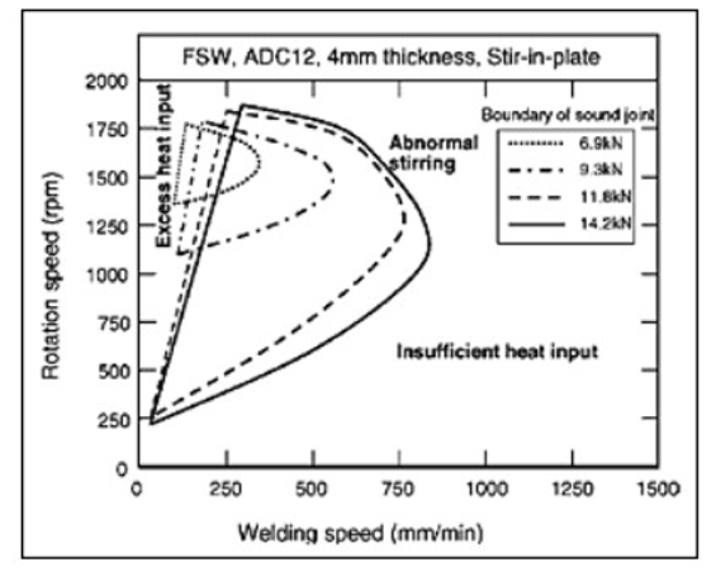
\includegraphics[width=\linewidth]{fig-janela-processo.png}
\fonte{Janela de processo: calor insuficiente, adequado e excessivo. Bezerra (2025)}
\end{column}
\end{columns}
\end{frame}

\begin{frame}[plain]
\centering
\vspace{0.6cm}

\includegraphics[height=1.2cm]{ita-logo.png}\par\vspace{0.6cm}
{\color{azulita}\LARGE\bfseries Obrigado!\par}
\vspace{0.4cm}{\color{azulita}\rule{0.3\linewidth}{0.6pt}}\par\vspace{0.4cm}
{\normalsize Rafael Lucas de Albuquerque Louvain\par}\vspace{2pt}
{\small\color{cinza}rafael.la.louvain@gmail.com\par}\vspace{2pt}
{\footnotesize\color{cinza}github.com/RafaellLouvain/TG-ITA-rafaellouvain\par}
\end{frame}

% =============================================================================
\appendix
\section{Reserva}
% =============================================================================
\begin{frame}{Reserva: validação por estudo da abordagem 2}
\begin{columns}[T,onlytextwidth]
\begin{column}{0.45\textwidth}
\begin{bullets}
  \item \textbf{Como funciona:} cada estudo sai inteiro para teste; o modelo é calibrado com os outros 13.
  \item \textbf{$V_{crit}$ estável:} 0,84 m/s em quase todas as rodadas (0,80 sem o estudo 6; 1,05 sem o estudo 11).
  \item \textbf{Erros concentrados:} estudos 6, 8, 10, 12 e 13, com vazios em velocidades altas ou soldas sãs em velocidades baixas.
  \item \textbf{Total:} 72 acertos em 108 soldas (66,7\%).
\end{bullets}
\end{column}
\begin{column}{0.52\textwidth}
\centering\scriptsize\setlength{\tabcolsep}{4pt}\renewcommand{\arraystretch}{0.9}
\begin{tabular}{ccccc}
\toprule
\textbf{Estudo} & \textbf{Soldas} & \textbf{Vazio} & \textbf{Acertos} & \textbf{$V_{crit}$ (m/s)} \\ \midrule
6 & 15 & 9 & 6 & 0,80 \\
7 & 7 & 3 & 4 & 0,84 \\
7b & 6 & 3 & 4 & 0,84 \\
8 & 3 & 1 & 1 & 0,84 \\
9 & 13 & 7 & 9 & 0,86 \\
10 & 6 & 3 & 3 & 0,84 \\
11 & 15 & 3 & 10 & 1,05 \\
12 & 5 & 3 & 3 & 0,84 \\
13 & 6 & 2 & 3 & 0,84 \\
14 & 13 & 2 & 13 & 0,84 \\
15 & 6 & 2 & 5 & 0,84 \\
16 & 8 & 2 & 6 & 0,84 \\
17 & 2 & 1 & 2 & 0,84 \\
18 & 3 & 2 & 3 & 0,84 \\ \bottomrule
\end{tabular}
\end{column}
\end{columns}
\end{frame}

\begin{frame}{Reserva: recalibração nos ensaios de Cintra}
\vspace{0.2cm}
\begin{bullets}
  \item \textbf{Limiar por acurácia:} sai acima de todos os ensaios (2,2 m/s); o índice prevê túnel em todos, com 85,0\% de acurácia de teste média, igual a prever sempre túnel.
  \item \textbf{Limiar por acurácia balanceada:} sai abaixo de todos os ensaios (0,16 m/s); acurácia balanceada de 42,8\%, próxima à de um sorteio.
  \item \textbf{Expoentes livres:} a regressão com $\omega$ e $v$ livres dá $+1{,}6$ para a rotação e $-1{,}6$ para o avanço: o risco de túnel cresce com a energia por comprimento, ao contrário do vazio frio, como também observou Bezerra (2025).
  \item \textbf{Leitura:} não existe rotação, dentro da faixa ensaiada, a partir da qual o túnel deixe de ocorrer.
\end{bullets}
\end{frame}

\end{document}
